\documentclass[]{article}
\usepackage{lmodern}
\usepackage{amssymb,amsmath}
\usepackage{ifxetex,ifluatex}
\usepackage{fixltx2e} % provides \textsubscript
\ifnum 0\ifxetex 1\fi\ifluatex 1\fi=0 % if pdftex
  \usepackage[T1]{fontenc}
  \usepackage[utf8]{inputenc}
\else % if luatex or xelatex
  \ifxetex
    \usepackage{mathspec}
  \else
    \usepackage{fontspec}
  \fi
  \defaultfontfeatures{Ligatures=TeX,Scale=MatchLowercase}
\fi
% use upquote if available, for straight quotes in verbatim environments
\IfFileExists{upquote.sty}{\usepackage{upquote}}{}
% use microtype if available
\IfFileExists{microtype.sty}{%
\usepackage{microtype}
\UseMicrotypeSet[protrusion]{basicmath} % disable protrusion for tt fonts
}{}
\usepackage[margin=1in]{geometry}
\usepackage{hyperref}
\hypersetup{unicode=true,
            pdftitle={Relatório para o Roteiro I de Modelagem Matemática em Finanças I},
            pdfauthor={Luiz Rodrigo Silva de Souza},
            pdfborder={0 0 0},
            breaklinks=true}
\urlstyle{same}  % don't use monospace font for urls
\usepackage{graphicx,grffile}
\makeatletter
\def\maxwidth{\ifdim\Gin@nat@width>\linewidth\linewidth\else\Gin@nat@width\fi}
\def\maxheight{\ifdim\Gin@nat@height>\textheight\textheight\else\Gin@nat@height\fi}
\makeatother
% Scale images if necessary, so that they will not overflow the page
% margins by default, and it is still possible to overwrite the defaults
% using explicit options in \includegraphics[width, height, ...]{}
\setkeys{Gin}{width=\maxwidth,height=\maxheight,keepaspectratio}
\IfFileExists{parskip.sty}{%
\usepackage{parskip}
}{% else
\setlength{\parindent}{0pt}
\setlength{\parskip}{6pt plus 2pt minus 1pt}
}
\setlength{\emergencystretch}{3em}  % prevent overfull lines
\providecommand{\tightlist}{%
  \setlength{\itemsep}{0pt}\setlength{\parskip}{0pt}}
\setcounter{secnumdepth}{0}
% Redefines (sub)paragraphs to behave more like sections
\ifx\paragraph\undefined\else
\let\oldparagraph\paragraph
\renewcommand{\paragraph}[1]{\oldparagraph{#1}\mbox{}}
\fi
\ifx\subparagraph\undefined\else
\let\oldsubparagraph\subparagraph
\renewcommand{\subparagraph}[1]{\oldsubparagraph{#1}\mbox{}}
\fi

%%% Use protect on footnotes to avoid problems with footnotes in titles
\let\rmarkdownfootnote\footnote%
\def\footnote{\protect\rmarkdownfootnote}

%%% Change title format to be more compact
\usepackage{titling}

% Create subtitle command for use in maketitle
\newcommand{\subtitle}[1]{
  \posttitle{
    \begin{center}\large#1\end{center}
    }
}

\setlength{\droptitle}{-2em}
  \title{Relatório para o Roteiro I de Modelagem Matemática em Finanças I}
  \pretitle{\vspace{\droptitle}\centering\huge}
  \posttitle{\par}
  \author{Luiz Rodrigo Silva de Souza}
  \preauthor{\centering\large\emph}
  \postauthor{\par}
  \predate{\centering\large\emph}
  \postdate{\par}
  \date{16 de abril de 2018}


\begin{document}
\maketitle

\emph{Observação:} o aplicativo que desenvolvi para essa atividade pode
ser testado em

\texttt{http://lurodrigo.com/mmfin1/bopm/}

\textbf{Atividade 2:} O valor de \(u\) será \(u_a^{\frac{T}{360N}}\).
Basta ver que \(u_d = u_a^{\frac{1}{360}}\). Tendo a taxa diária, o
valor de \(u\) deve ser tal que \(u^N = u_d^T\), e aí obtemos a fórmula
acima. Utilizando o mesmo raciocínio, encontramos
\(r = (1+r_a)^{\frac{T}{360N}} - 1\).

\textbf{Atividade 3:} Tanto faz, pois as transformação
\(u \mapsto u^{\frac{1}{360}}\) e
\(r \mapsto (1 + r)^{\frac{1}{360}} - 1\) são crescentes, ou seja,
preservam as comparações.

Aqui abaixo estão exemplos de random walks com todos os parâmetros
iguais, exceto pelo \(N\), que é 10 ou 100.

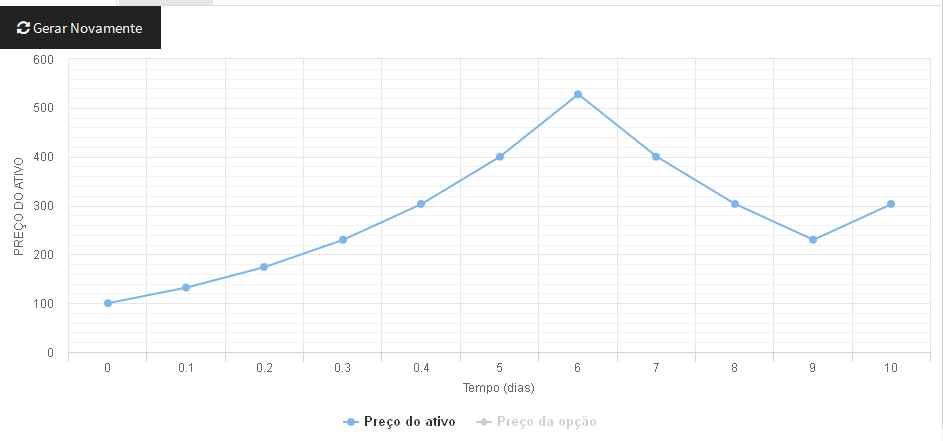
\includegraphics{grafico1.png} 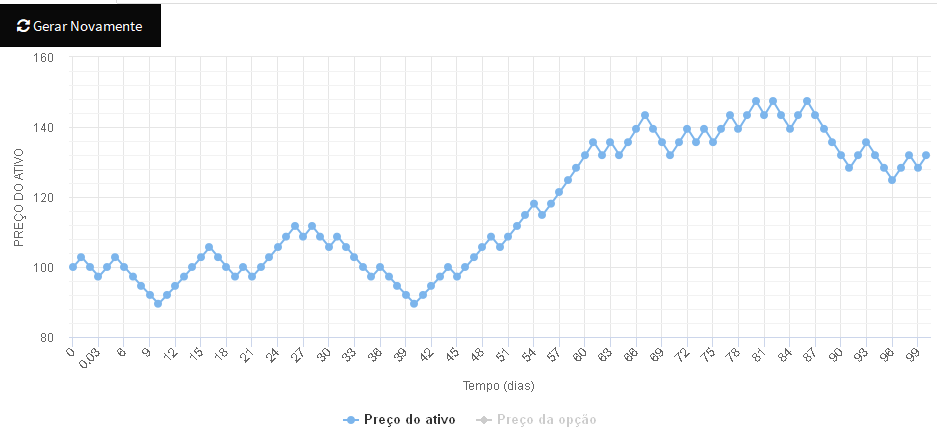
\includegraphics{grafico2.png}

Naturalmente, além dos resultados diferentes dos lançamentos de moeda, a
diferença está na \emph{resolução} do modelo: um modelo com N maior
contempla uma quantidade maior de valores possíveis para o valor final
do ativo.

\textbf{Atividade 4:} Fiz esse gráfico para o exemplo 1.2.2 do livro. A
diferença está somente no payoff, que é de uma call option e não de uma
loopback option. O gráfico mantém os parâmetros fixos, exceto N, que
varia. Parece haver convergência para um valor não-nulo à medida que N
aumenta.

\begin{figure}
\centering
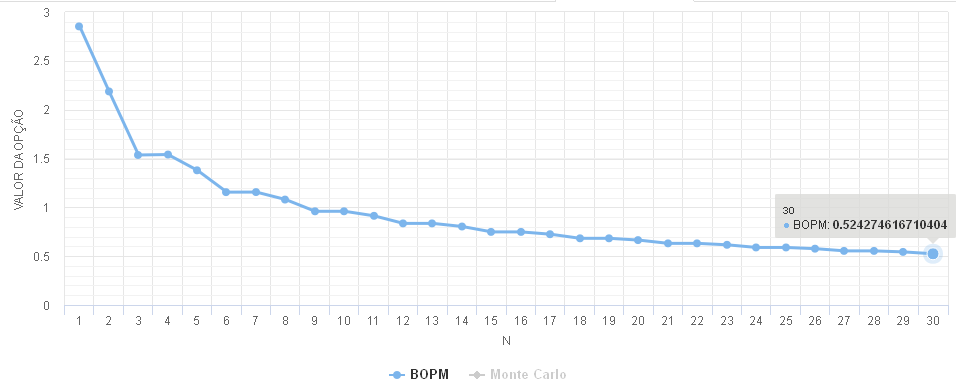
\includegraphics{grafico3.png}
\caption{}
\end{figure}

\textbf{Atividade 5:}

\textbf{Atividade 6:}


\end{document}
